\documentclass[border=2pt]{standalone}
\usepackage{tikz}
\usetikzlibrary{arrows.meta,chains,%
                    decorations.pathreplacing}
\usetikzlibrary{matrix,positioning,arrows.meta,arrows}

\tikzset{
mymat/.style={
  matrix of nodes,
  nodes in empty cells,
  text height=2.5ex,
  text depth=0.75ex,
  text width=3.25ex,
  align=center,
  column sep=-\pgflinewidth
  }
}
\tikzset{
  rows/.style 2 args={
    sub@rows/.style={row ##1 column #2/.style={nodes={rectangle,draw=black}}},
    sub@rows/.list={#1}
  },
  box/.style 2 args={
    sub@box/.style={rows={#1}{##1}},
    sub@box/.list={#2}
  }
}
\begin{document}

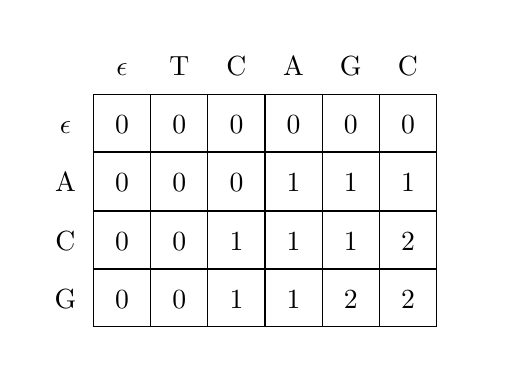
\begin{tikzpicture}[>=latex]
\matrix[mymat,anchor=west,
    box={2, 3, 4, 5}{2, 3, 4, 5, 6, 7}]
at (0,0) 
(mat1)
{ 
   & $\epsilon$ & T & C & A & G & C & \\
  $\epsilon$ & 0 & 0 & 0 & 0 & 0 & 0\\
  A & 0 & 0 & 0 & 1 & 1 & 1 & \\
  C & 0 & 0 & 1 & 1 & 1 & 2 & \\
  G & 0 & 0 & 1 & 1 & 2 & 2 & \\ };
\end{tikzpicture}

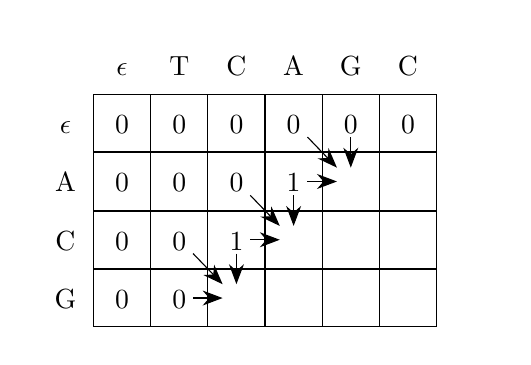
\begin{tikzpicture}[>=latex]
\matrix[mymat,anchor=west,
    box={2, 3, 4, 5}{2, 3, 4, 5, 6, 7}]
at (0,0) 
(mat1)
{ 
   & $\epsilon$ & T & C & A & G & C & \\
  $\epsilon$ & 0 & 0 & 0 & 0 & 0 & 0 \\
  A & 0 & 0 & 0 & 1 &  &  & \\
  C & 0 & 0 & 1 &  &  &  & \\
  G & 0 & 0 &  &  &  &  & \\ };


\begin{scope}
\coordinate(dp1-4-5) at([xshift=-5pt,yshift=5pt]mat1-4-5.center);
\coordinate(dp2-4-5) at([yshift=5pt]mat1-4-5.center);
\coordinate(dp3-4-5) at([xshift=-5pt]mat1-4-5.center);

\coordinate(odp3-3-4) at([xshift=5pt,yshift=-5pt]mat1-3-4.center);
\coordinate(odp3-3-5) at([yshift=-5pt]mat1-3-5.center);
\coordinate(odp3-4-4) at([xshift=5pt]mat1-4-4.center);

\draw[-{Stealth[scale=1.5]}] (odp3-3-4) -- (dp1-4-5);
\draw[-{Stealth[scale=1.5]}] (odp3-3-5) -- (dp2-4-5);
\draw[-{Stealth[scale=1.5]}] (odp3-4-4) -- (dp3-4-5);
\end{scope}

\begin{scope}
\coordinate(dp1-4-5) at([xshift=-5pt,yshift=5pt]mat1-3-6.center);
\coordinate(dp2-4-5) at([yshift=5pt]mat1-3-6.center);
\coordinate(dp3-4-5) at([xshift=-5pt]mat1-3-6.center);

\coordinate(odp3-3-4) at([xshift=5pt,yshift=-5pt]mat1-2-5.center);
\coordinate(odp3-3-5) at([yshift=-5pt]mat1-2-6.center);
\coordinate(odp3-4-4) at([xshift=5pt]mat1-3-5.center);

\draw[-{Stealth[scale=1.5]}] (odp3-3-4) -- (dp1-4-5);
\draw[-{Stealth[scale=1.5]}] (odp3-3-5) -- (dp2-4-5);
\draw[-{Stealth[scale=1.5]}] (odp3-4-4) -- (dp3-4-5);
\end{scope}

\begin{scope}
\coordinate(dp1-4-5) at([xshift=-5pt,yshift=5pt]mat1-5-4.center);
\coordinate(dp2-4-5) at([yshift=5pt]mat1-5-4.center);
\coordinate(dp3-4-5) at([xshift=-5pt]mat1-5-4.center);

\coordinate(odp3-3-4) at([xshift=5pt,yshift=-5pt]mat1-4-3.center);
\coordinate(odp3-3-5) at([yshift=-5pt]mat1-4-4.center);
\coordinate(odp3-4-4) at([xshift=5pt]mat1-5-3.center);

\draw[-{Stealth[scale=1.5]}] (odp3-3-4) -- (dp1-4-5);
\draw[-{Stealth[scale=1.5]}] (odp3-3-5) -- (dp2-4-5);
\draw[-{Stealth[scale=1.5]}] (odp3-4-4) -- (dp3-4-5);
\end{scope}

\end{tikzpicture}

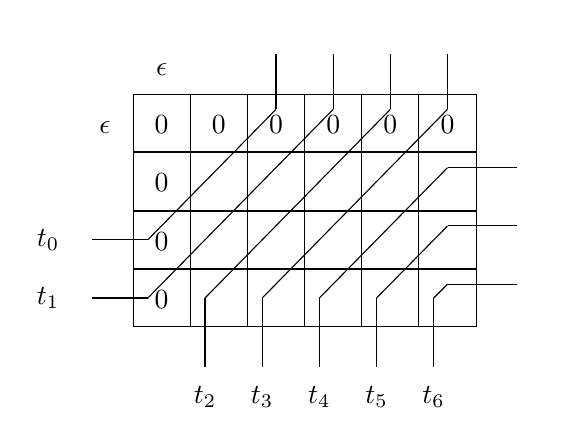
\begin{tikzpicture}[>=latex]
\matrix[mymat,anchor=west,
    box={2, 3, 4, 5}{2, 3, 4, 5, 6, 7}]
at (0,0) 
(mat1)
{ 
   & $\epsilon$ &  &  &  &  &  & \\
  $\epsilon$ & 0 & 0 & 0 & 0 & 0 & 0 \\
   & 0 &  &  &  &  &  & \\
   & 0 &  &  &  &  &  & \\
   & 0 &  &  &  &  &  & \\ };

\begin{scope}
\coordinate(bup) at([yshift=5pt]mat1-2-4.center);
\coordinate(bleft) at([xshift=-5pt]mat1-4-2.center);
\coordinate(bup-f) at([yshift=25pt]mat1-2-4.center);
\coordinate(bleft-f) at([xshift=-25pt]mat1-4-2.center);

\draw (bup) -- (bleft);
\draw (bup) -- (bup-f);
\draw (bleft) -- (bleft-f);
\node[left=of bleft]{$t_0$};
\end{scope}

\begin{scope}
\coordinate(bup) at([yshift=5pt]mat1-2-5.center);
\coordinate(bleft) at([xshift=-5pt]mat1-5-2.center);
\coordinate(bup-f) at([yshift=25pt]mat1-2-5.center);
\coordinate(bleft-f) at([xshift=-25pt]mat1-5-2.center);

\draw (bup) -- (bleft);
\draw (bup) -- (bup-f);
\draw (bleft) -- (bleft-f);
\node[left=of bleft]{$t_1$};
\end{scope}

\begin{scope}
\coordinate(bup) at([yshift=5pt]mat1-2-6.center);
\coordinate(bleft) at([xshift=-5pt]mat1-5-3.center);
\coordinate(bup-f) at([yshift=25pt]mat1-2-6.center);
\coordinate(bleft-f) at([xshift=-5pt,yshift=-25pt]mat1-5-3.center);

\draw (bup) -- (bleft);
\draw (bup) -- (bup-f);
\draw (bleft) -- (bleft-f);
\node[below=of bleft]{$t_2$};
\end{scope}

\begin{scope}
\coordinate(bup) at([yshift=5pt]mat1-2-7.center);
\coordinate(bleft) at([xshift=-5pt]mat1-5-4.center);
\coordinate(bup-f) at([yshift=25pt]mat1-2-7.center);
\coordinate(bleft-f) at([xshift=-5pt,yshift=-25pt]mat1-5-4.center);

\draw (bup) -- (bleft);
\draw (bup) -- (bup-f);
\draw (bleft) -- (bleft-f);
\node[below=of bleft]{$t_3$};
\end{scope}

\begin{scope}
\coordinate(bup) at([yshift=5pt]mat1-3-7.center);
\coordinate(bleft) at([xshift=-5pt]mat1-5-5.center);
\coordinate(bup-f) at([yshift=5pt, xshift=25pt]mat1-3-7.center);
\coordinate(bleft-f) at([xshift=-5pt,yshift=-25pt]mat1-5-5.center);

\draw (bup) -- (bleft);
\draw (bup) -- (bup-f);
\draw (bleft) -- (bleft-f);
\node[below=of bleft]{$t_4$};
\end{scope}

\begin{scope}
\coordinate(bup) at([yshift=5pt]mat1-4-7.center);
\coordinate(bleft) at([xshift=-5pt]mat1-5-6.center);
\coordinate(bup-f) at([yshift=5pt, xshift=25pt]mat1-4-7.center);
\coordinate(bleft-f) at([xshift=-5pt,yshift=-25pt]mat1-5-6.center);

\draw (bup) -- (bleft);
\draw (bup) -- (bup-f);
\draw (bleft) -- (bleft-f);
\node[below=of bleft]{$t_5$};
\end{scope}

\begin{scope}
\coordinate(bup) at([yshift=5pt]mat1-5-7.center);
\coordinate(bleft) at([xshift=-5pt]mat1-5-7.center);
\coordinate(bup-f) at([yshift=5pt, xshift=25pt]mat1-5-7.center);
\coordinate(bleft-f) at([xshift=-5pt,yshift=-25pt]mat1-5-7.center);

\draw (bup) -- (bleft);
\draw (bup) -- (bup-f);
\draw (bleft) -- (bleft-f);
\node[below=of bleft]{$t_6$};
\end{scope}


\end{tikzpicture}

\end{document}